\documentclass{article}
\usepackage{graphicx}
\usepackage{float}
\usepackage{amsmath}
\usepackage{amsfonts}
\usepackage{amssymb}
\usepackage{hyperref}
\usepackage{esint}
\usepackage[utf8]{inputenc}
\usepackage[a4paper, portrait, margin=0.75in]{geometry}
\setlength\parindent{0pt}
\usepackage[italian]{babel}
\usepackage{tikz} 





\hypersetup{
    colorlinks=true,
    linkcolor=black,
    filecolor=magenta,
    urlcolor=blue,
    pdftitle={Tecnologie internet},
    pdfpagemode=FullScreen,
}


\begin{document}
    \author{kanopo}
    \title{APPLICAZIONI INDUSTRIALI ELETTRICHE ED ELETTRONICA (MODULO 2)}
    \date{2022}

    \maketitle
    \tableofcontents

    \listoffigures
    \listoftables

    \section{Introduzione all'elettronica}
\subsection{Trasduttori}
I trasduttori sono dispositivi che mettono in contatto la realtà e l'elettonica.

ne esistono di due famiglie:
\begin{itemize}
    \item sensori
    \item trasduttori
\end{itemize}

I sensori trasformano grandezze fisiche in elettriche, mentre i trasduttori utilizzano le grandezze elettriche per trasformarle in grandezzze fisiche.

\subsection{Digitale vs analogico}
\begin{itemize}
    \item grande potenza di calcolo ed eleaborazione del segnale
    \item maggior robustezza ai disturbi
    \item minor sensibilità alla temperatura
\end{itemize}

\subsection{Analogico vs digitale}
\begin{itemize}
    \item in natura le grandezze fisiche sono descrivibili come segnali analogici
    \item sensori e attuatori
    \item per la conversione da analogico a digitale e viceversa, si usano circuiti DAC e ADC
\end{itemize}

\subsection{ADC(Convertitore analogico digitale)}
\begin{itemize}
    \item viene fissata la tensione di fondo scala ($V_{fs}$)
    \item la tensione d'ingresso analogica viene convertita nel valore più vicino numero a n-bit
    \item maggiore è il numero di bit usati per la conversione e maggiore è la precisione del ADC(si perdono meno informazioni nella conversione)(minor errore di quantizzazione).
\end{itemize}


\subsection{DAC(convertitore digitale analogico)}
la tensione in uscita è:
\begin{equation*}
    V_O = (\sum_n^{+\infty} b_n 2^{-n}) V_{fs}
\end{equation*}
\begin{equation*}
    V_O = (b_12^{-1} + b_22^{-2} + \dots + b_n2^{-n}) V_{fs}
\end{equation*}

Scritto in due maniere(sero uguali)




    \section{Semiconduttori}

\subsection{Caratteristiche}
\begin{itemize}
    \item Resistività ($\rho$) intermedia tra isolanti e conduttori
    \item possibilità di variare $\rho$ mediante il drogaggio
    \item due portatori di carica(elettroni e lacune)
\end{itemize}

\subsection{Drogaggio di un semiconduttore}
Sostanzialmente si mettono atomi di diverso tipo nel composto che va a formare il semiconduttore finale.

Quando parliamo di silicio, distinguiamo silicio-p e silicio-n.
\begin{itemize}
    \item droganti di tipo n: elementi del 5 gruppo(5 elettroni esterni o di valenza)
    \item droganti di tipo p: 3 elettroni di valenza 
\end{itemize}


Nei composti drogati di tipo n, si forma un atomo libero di muoversi e nei composti di tipo p si ha una mancanza di un atomo(quidni una lacuna).


\subsection{Correnti di "drift"}

Per campi elettrici moderati esiste una relazione lineare tra intensità del campo 
e velocità media dei portatori di carica.

Ci sono materiali con un'alta mobilità delle cariche($\mu$).

La corrente di drifpt penso sia legata alla conducibilità del materiale.

\subsection{Diffusione}
Simile ai gas, i semiconduttori cercano di avere un equilibrio di cariche al propro interno.



    \section{Diodo}
\subsection{Diodo a giunzione PN}

Il diodo è formato da due parti, una parte drogata di tipo p e una drogata di tipo n.

Questa costruzione forma ua forza che impedisce il passaggio di cariche nei diodi perchè si oppone 
a quello che dovrebbe essere il normale fluire delle  cariche avendo una parte positiva e una negativa.

Fra la parte P e quella N si trova la "regione svuotata".

\subsection{Diodo polarizzato in diretta}

la tensione applicata dall'esterno si localiza tutta ai capi della regione svuotata, la corrente di diffusione prevade su quella di drift e c'è il passaggio delle cariche.


Tendenzialmente la tensione da vincere per permettere il fluire della corrente è di $V_T = 0.7V$ ma varia in base ai materiali impiegati e alle temperature.

\subsection{Diodo polaizzato in inversa}


La barrriera di potenziale si alza un \textbf{botto}.

Per correnti molto la giunzione funziona come interruttore aperto, però se si continua ad
aumentare la corrente si incombe nella corrente di breakdown.

\subsubsection{Breakdown a valanga}
\begin{itemize}
    \item vengono iniettati elettroni nella regione svuotata
    \item forte campo elettrico nella regione svuotata
    \item l'elettrone acquista elevata forza cinetica
    \item collisione con atomo nel reticolo
    \item un'elettrone dell'atomo si libera e applica energia ad altri legami
    \item si crea una valanga dove esplode tutto
    \item il diodo è cafuddato
\end{itemize}


    \section{BJT(Transistore bipolare a giunzione)}


    \section{Transistor MOSFET(Metal-Oxide Semiconductor Field Effect Transistor)}

\begin{figure}[H]
    \centering
    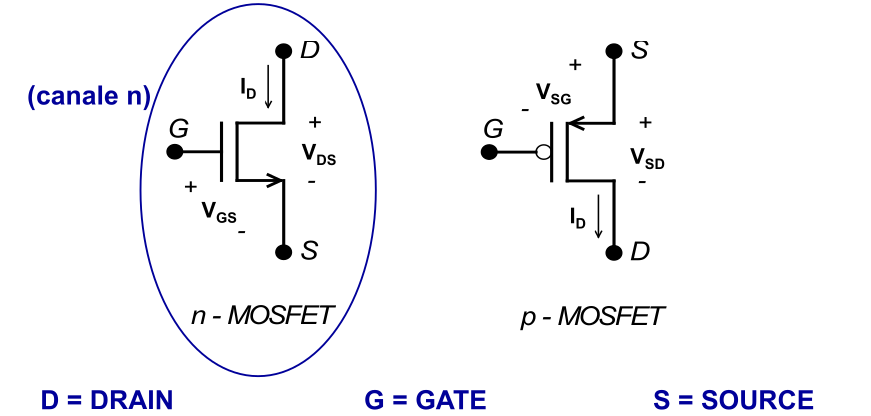
\includegraphics[width=0.5\linewidth]{2 - dispositivi elettronici/imgs/Screenshot from 2022-06-14 23-25-50.png}
\label{fig:MOSFET}
\caption{MOSFET}
\end{figure}

\subsection{Capacità MOS: accumulazione}

\begin{figure}[H]
    \centering
    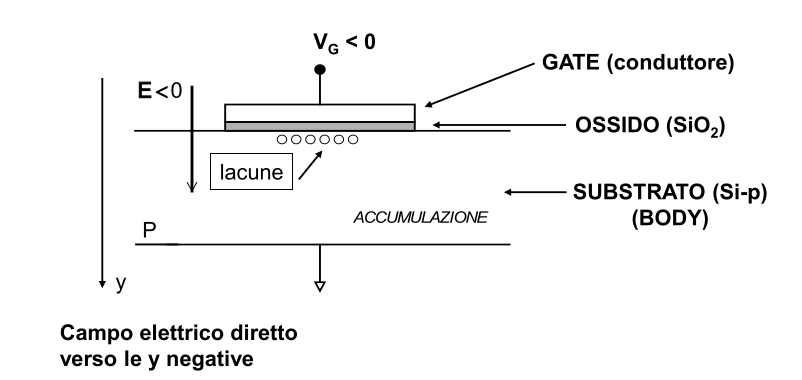
\includegraphics[width=0.5\linewidth]{2 - dispositivi elettronici/imgs/Screenshot from 2022-06-15 11-23-56.png}
    \caption{MOS accumulazione}
    \label{fig:MOS_acc}
\end{figure}

L'accumulazione è l'aumento di concentrazione di lacune sotto l'ossido del gate.

\subsection{Capacità MOS: svuotamento}

\begin{figure}[H]
    \centering
    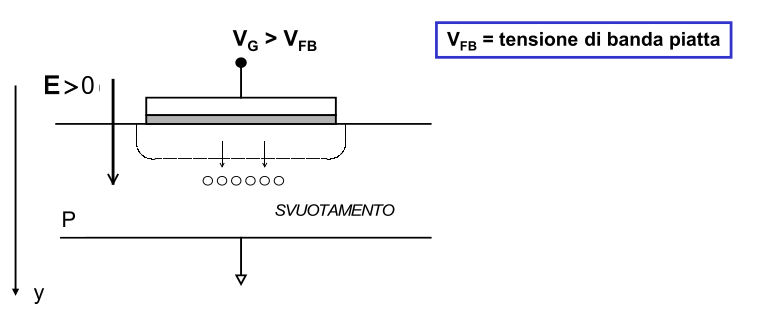
\includegraphics[]{2 - dispositivi elettronici/imgs/Screenshot from 2022-06-15 11-30-59.png}
    \label{fig:MOS_svuotamento}
    \caption{MOS svuotamento}
\end{figure}

Le lacune vengono allontanate dal campo elettrico e viene 
creata una zona svuotata sotto l'ossido del gate.
\end{document}